%!TEX root = ../thesis.tex
%*******************************************************************************
%****************************** Second Chapter *********************************
%*******************************************************************************

\chapter{Preliminaries}

\ifpdf
    \graphicspath{{Chapter2/Figs/Raster/}{Chapter2/Figs/PDF/}{Chapter2/Figs/}}
\else
    \graphicspath{{Chapter2/Figs/Vector/}{Chapter2/Figs/}}
\fi


\section{Machine Learning}
\label{preliminaries:machine_learning}

Machine learning is a field in computer science that we try teaching the computers to do tasks without explicitly programmed \citep{samuel2000some, koza1996automated}. Machine learning is strongly associated with computational statistics, which explores data and builds algorithms that could find patterns in data and make predictions. More formal definition of the algorithms used in the machine learning is provided by Mitchell ``A computer program is said to learn from experience E with respect to some class of tasks T and performance measure P if its performance at tasks in T, as measured by P, improves with experience E`` \citep{mitchell1997machine}.

Typically, tasks in machine learning can be grouped into three wide categories \citep{russell1995modern}:

\begin{itemize}
\item Supervised learning: the given data contains input values and their desired output values, the aim of algorithms in supervised learning is to find a general rule that maps inputs to outputs. In this thesis we are focus on the supervised learning approach for our fraud detection problem,
\item Unsupervised learning: there are no desired outputs in the dataset, it means that we give the learning algorithms freely to explore a hidden structure of the data,
\item Reinforcement learning: this kind of learning is slightly different with the above, reinforcement learning builds a dynamic environment then let a computer interacts with it to perform a certain goal, after each action a feedback is provided to the computer as a reward or a punishment.
\end{itemize}


Supervised learning is a most common task in the world and can be seen as a function from labeled training data \citep{mohri2012foundations}. Given a set of $N$ data points of a form ${(x_1, y_1), \dots, (x_N, y_N)}$ such that $x_i$ is a attribute vector of the i-th data point and $y_i$ is its desired output, a supervised learning algorithm is a function $g: X \rightarrow Y$, where $X$ is an input space (matrix of attribute vectors) and $Y$ is a output space (matrix of desired outputs). Typically the function $g$ is in a function space $G$, or we could represent $g$ as a scoring function $f: X \times Y \rightarrow \mathbb{R}$ such that function $f$ will return the output value $y$ which has the highest score $g(x) = argmax_y f(x, y)$. For example, $g$ could be a conditional probability model $g(x) = P(y \mid x)$, e.g. logistic regression \citep{walker1967estimation, cox1958regression}, or $f$ could takes a form of a join t probability model $f(x, y) = P(x, y)$, e.g. naive Bayes \citep{russell1995modern}.

In order to measure a performance of learning function, we could define a loss function $L: Y \times Y \rightarrow \mathbb{R}$ and a risk $R(g)$ of learning function $g$ is defined as an expected loss of function $g$ which could be estimated by:

\begin{equation}
\widehat{R} (g) = \dfrac{1}{N} \sum_i L(y_i, g(x_i))
\end{equation}

\subsection*{Decision tree learning}

A decision tree learning is one common approach in data mining \citep{rokach2014data}, it aims to create a model that predicts values like making a decision from a tree-based analysis. An example is shown in the figure \ref{img:titanic_survival_decision_tree} \citep{decision_tree_learning}.

\begin{figure}
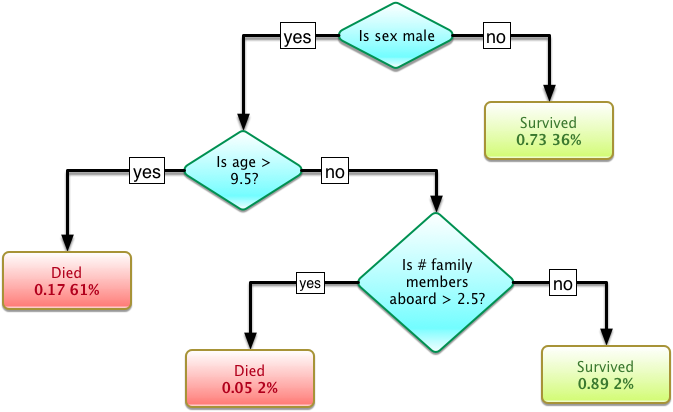
\includegraphics[scale=0.4]{Images/Titanic_Survival_Decison_Tree_SVG.png}
\centering
\caption{A tree showing survival of passengers on the Titanic}
\label{img:titanic_survival_decision_tree}
\end{figure}

A tree learner could classify the data points by splitting the input dataset into subsets based on a given criterion. The splitting process at each node is repeated in a recursive procedure until all data points are classified. There are two kinds of decision trees:

\begin{itemize}
\item Regression tree: create a tree to predict the desired output as a real number,
\item Classification tree: an analysis aims to predict a categorical output.
\end{itemize}

A term Classification and Regression Tree (CART) analysis is used to refer to both the above analysis \citep{breiman1984classification}. There are many decision tree algorithms, including:

\begin{itemize}
\item ID3 (Iterative Dichotomiser 3) \citep{quinlan1986induction},
\item C4.5: an extension of ID3 algorithm \citep{quinlan2014c4}.
\end{itemize}

Algorithms for constructing decision trees use different metrics for measuring which is the best feature to split the dataset. These measures compute the homogeneity of the output values within the subsets, some common measures in decision tree learning is Entropy, Information Gain, and Gini.


\subsection*{Ensemble learning}

In machine learning, ensemble learning is a method combines multiple learning algorithms to obtain better accuracy than from any individual algorithms \citep{opitz1999popular, rokach2010ensemble}. The term ensemble is usually reserved for methods that generate multiple hypotheses using the same base learner. There are three common types of ensemble learning, such as:


\subparagraph{Bootstrap aggregating (bagging)}

An ensemble technique is bootstrap aggregating which is usually called bagging (see figure \ref{img:bagging_ensemble}), it combines multiple learnings via their equal weight votes. In order to support the model variance, bagging trains each model from a randomly drawn subset. And a famous example of bagging is the Random Forest algorithm which uses random decision trees as base learners.


\begin{figure}
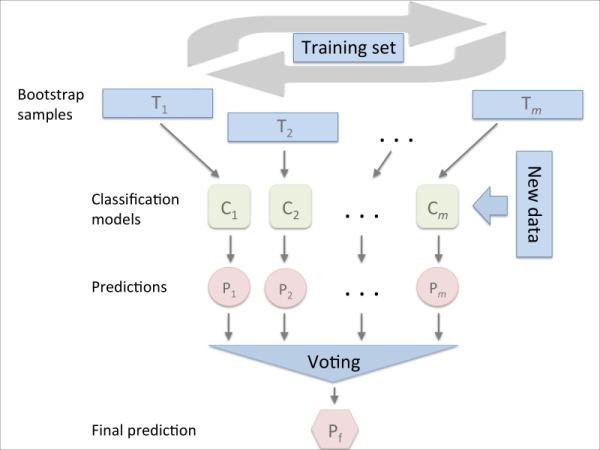
\includegraphics[scale=0.4]{Images/bagging.jpg}
\centering
\caption{Bagging ensemble \citep{raschka2015python}}
\label{img:bagging_ensemble}
\end{figure}


\subparagraph{Boosting}

Similar with the bagging ensemble, boosting is an incremental algorithm that will train each new model to underline the data points that previous models mis-classified (see figure \ref{img:boosting_ensemble}). Boosting could have a better accuracy than bagging in some cases, however it also tends to overfit to the training data. A most common boosting algorithm is Adaboost \citep{freund1999short}.


\begin{figure}
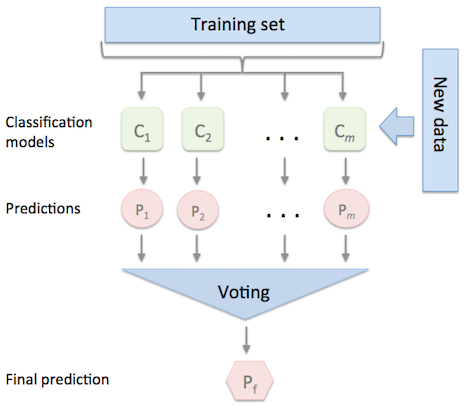
\includegraphics[scale=0.4]{Images/boosting.png}
\centering
\caption{Boosting ensemble \citep{raschka2015python}}
\label{img:boosting_ensemble}
\end{figure}


\subparagraph{Stacking}

Slightly different with these above techniques, stacking is a supervised learning algorithm that uses the predictions of several other learning algorithms as an input dataset to makes the final prediction (see figure \ref{img:stacking_ensemble}). All of the other algorithms are trained using the given dataset independently, then a combiner algorithm is trained on that which can be any algorithm. Therefore, stacking can theoretically represent any of the ensemble techniques, although in practice we often use the Logistic Regression or Linear Regression as the combiner.


\begin{figure}
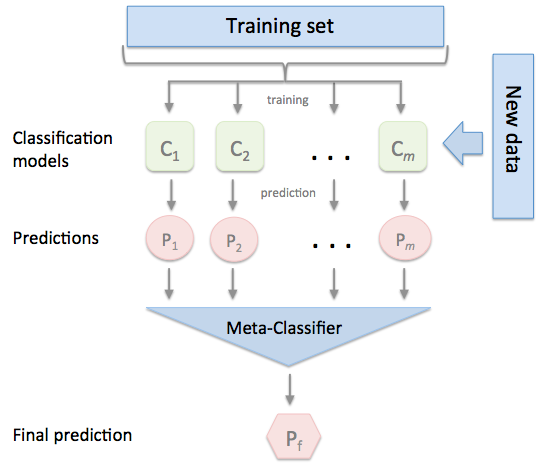
\includegraphics[scale=0.4]{Images/stacking.png}
\centering
\caption{Stacking ensemble \citep{raschka2015python}}
\label{img:stacking_ensemble}
\end{figure}


\subsection*{Random Forest}

Random Forest \citep{breiman2001random} or random decision forests \citep{ho1995random, ho1998random} are an ensemble learning method for classification or regression that perform by constructing many trees, e.g. decision trees, then combine these results to makes final output values as a mode of the classes for classification tasks or a mean prediction for regression tasks. The Random Forest model based on two elements:


\begin{enumerate}
\item Base learner: each tree in the forest is the base learner, typically it is a weak learner with high variance,
\item Ensemble learning: combine the results of several weak learners to make a final prediction.
\end{enumerate}


The Decision Tree above that are grown very deep tend to overfit their training sets, i.e. have a low bias, but very high variance. We use the tree-based method as the base learner by its strength, and to handle its weakness we combine all of the predictions via ensemble learning. This method is called Random Forest, it can formulate the algorithm as the following statement: given a dataset $X = x_1, \dots, x_n$ with $n$ data points and respectively desired output values $Y = y_1, \dots, y_n$, bagging repeatedly $B$ times selects a random sample from the dataset $X$ then training trees on these samples.


\begin{algorithm}
   \caption{Tree bagging}
    \begin{algorithmic}
      \Function{bagging}{$X, Y, B$}

        \For{$b = 1$ to ${B}$}
            \State $(X_b, Y_b)$ is samples from $(X, Y)$ which have $n$ data points
            \State Train a classification or regression tree $f_b$ on $X_b, Y_b$
        \EndFor
        
       \EndFunction

\end{algorithmic}
\end{algorithm}


The authors of Random Forest have proposed using an average function to makes the final prediction in regression tasks or takes the majority vote in classification tasks \citep{breiman2001random}. However, there is no standard function as a combiner, thus we are free to choose the combination function. This bootstrapping procedure could decrease the variance of the model without increasing the bias. In order to estimate the uncertainty of the prediction, it could be computed as a standard deviation of the predictions from all the individual trees:

\begin{equation}
\sigma = \sqrt{ \dfrac{ \sum_{b=1}^B ( f_b(x) - \hat{f} ) }{ B - 1 } }
\end{equation}

Random Forest uses the above bagging algorithm with only one difference, it uses a modified tree that selects a random subset of the features to split a current subset data. Typically, the dataset has $p$ features then for a classification problem $\sqrt{p}$ features will be used in each split and for regression problems the inventor recommends that we should use $p/3$ as the number of features \citep{friedman2001elements}.


\section{Measurement}
\label{measurement_premilinaries}

The fraud detection problem is the classification task and in order to measure how well of the classifiers, there are many metrics could be used to evaluate the algorithms. In this section, we will review some common metrics which are typically used in classification tasks.


\subsection*{Accuracy}

Accuracy is a measure of statistical variablity which represent a percentage of correct predictions on the total number of cases examined. In the fields of science and engineering, the accuracy of a measurement system is the degree of closeness of measurements of a quantity to that quantity's true value \citep{bipm2008international}. Consider 2 sets with $n$ data points: the true labels from the given dataset $Y = {y_1, \dots, y_n}$ and our predicted values $\hat{Y} = {\hat{y_1}, \dots, \hat{y_n}}$, the accuracy is:

\begin{equation}
accuracy = \dfrac{ 1 }{ n } \sum_{i = 1}^n \mbox{1\hspace{-4.25pt}\fontsize{12}{14.4}\selectfont\textrm{1}}_{ y_i = \hat{y_i} }
\end{equation}


\subsection*{Precision and recall}

In pattern recognition, information retrieval and binary classification, precision and recall are two common metrics. Precision (also called positive predictive value) is the fraction of relevant data points among the given data points, and recall (also known as sensitivity) is the fraction of relevant data points that have been retrieved over the total amount of relevant data points (see figure \ref{img:precision_and_recall}).


\begin{figure}
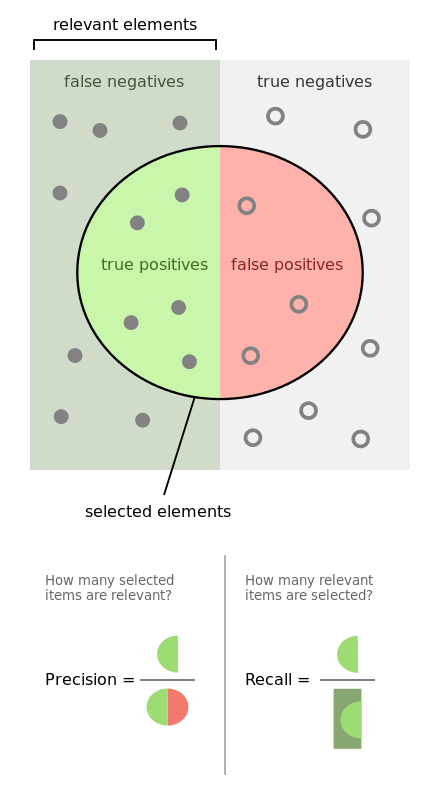
\includegraphics[scale=0.35]{Images/Precisionrecall.png}
\centering
\caption{Precision and recall \citep{wiki2018precision_recall}}
\label{img:precision_and_recall}
\end{figure}


In the information retrieval contexts, precision and recall were defined by Perry, Kent \& Berry (1955) \citep{perry1955machine} as a set of retrieved elements and a set of relevant elements. Precision is the fraction of retrieved documents that are relevant to the query:


\begin{equation}
\text{precision} = \dfrac{ \mid {\text{relevant elements}} \cap {\text{retrieved elements}} \mid }{ \mid {\text{retrieved elements}} \mid }
\end{equation}


And the recall is the fraction of the relevant elements that are successfully retrieved:


\begin{equation}
\text{precision} = \dfrac{ \mid {\text{relevant elements}} \cap {\text{retrieved elements}} \mid }{ \mid {\text{relevant elements}} \mid }
\end{equation}


In the classification tasks, considers four terms true positives (TP), true negatives (TN), false positives (FP), and false negatives (FN). Precision and recall are defined as \citep{olson2008advanced}:


\begin{equation}
\text{precision} = \dfrac{ TP }{ TP + FP }
\end{equation}


\begin{equation}
\text{recall} = \dfrac{ TP }{ TP + FN }
\end{equation}


\subsection*{Receiver operating characteristic (ROC)}

A receiver operating characteristic curve is a graphical plot which is created by plotting the true positive rate (TPR) against the false positive rate (FPR) at various threshold settings. ROC analysis provides tools to select a possible optimal threshold for models, an example ROC curve plot of three predictors of peptide cleaving in the proteasome is shown in figure \ref{img:roc_curve}.

\begin{figure}
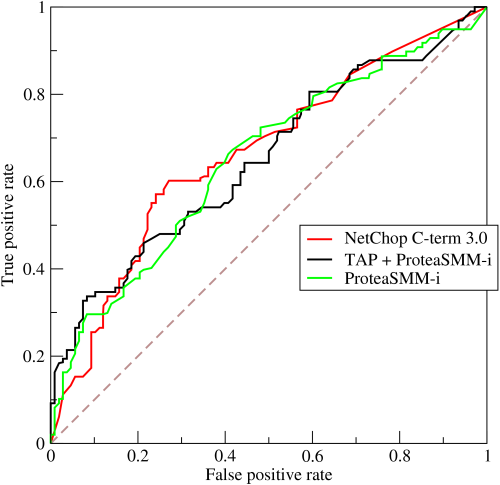
\includegraphics[scale=2.5]{Images/Roccurves.png}
\centering
\caption{ROC curve of three predictors of peptide cleaving in the proteasome \citep{wiki2018roc}}
\label{img:roc_curve}
\end{figure}


\subsection*{Area under the ROC curve (AUC)}

We cannot compare classifiers base on the ROC because the ROC curve is just a graphical plot. In order to represent ROC performance as a single scala, a common method is to calculate the area under the ROC curve (AUC for short). Because the AUC is a size of the area of the unit square, therefore the AUC value will always be between 0 and 1. However, random guessing produces an area of 0.5, no realistic classifier should have an AUC less than 0.5 then it makes the baseline performance for all classifiers is 0.5. In summary, the AUC metric is a measure of how much the ROC curve is close to the point of perfect classification.

The AUC metric usually used in machine learning community for model comparison \citep{hanley1983method}. However, in practice researchers recently noticed that AUC was quite noisy as a classification measure \citep{hanczar2010small} and some other studies have other significant problems in model comparison \citep{lobo2008auc, hand2009measuring}.

\subsection*{F-score}

$F_1$ score (also F-score or F-measure) is a measure that considers both precision and recall by taking a harmonic average of these metrics.


\begin{equation}
F_1 = 2 \cdot \dfrac{ \text{precision} \cdot \text{recall} }{ \text{precision} + \text{recall} }
\end{equation}


A general formula of F-score for any positive real $\beta$ is:


\begin{equation}
F_\beta = (1 + \beta^2) \cdot \dfrac{ \text{precision} \cdot \text{recall} }{ (\beta^2 \cdot \text{precision}) + \text{recall} }
\end{equation}


Van Rijsbergen et al. \citep{van1979information} interpret $F_\beta$ that "measures the effectiveness of retrieval with respect to a user who attaches $\beta$ times as much importance to recall as precision". In practice, the F-score metric is often used in machine learning when the dataset is imbalanced because it isn't affected by the imbalance problem.